\chapter{Project Management}
\label{chapter:teamplan}
Effective communication is the cornerstone of any successful project, since teamwork and coordination are paramount. A well-structured \textbf{Team Communication Plan} is essential to ensure that all team members are aligned, informed, and working efficiently towards common goals. \\
This chapter introduces the key components of the communication strategy, designed to facilitate seamless collaboration, streamline information sharing, and enhance overall project management. By leveraging a combination of modern tools and platforms, the aim is to create a robust communication framework that will support the project team throughout the development process, from initial planning to final delivery. \\
The following sections will explore each aspect of the communication plan, highlighting how various technologies can be utilized to foster transparency, productivity, and cohesion within the engineering team.

\section{Communication Tools and Platforms}
\label{section:comunication_tools}

\begin{itemize}
    \item \textbf{GitHub: } Utilized for code development, version control, and collaboration among team members. It provides a centralized repository for storing and managing the project's source code, facilitating seamless collaboration and code review processes.
    \item \textbf{OneDrive \& Overleaf: } For collaborative documentation development, the team will use OneDrive and Overleaf. These platforms allow for real-time editing and version control of project documents, ensuring that all team members have access to the most up-to-date information.
    \item \textbf{Jira: } Will serve as the primary tool for project organization and management. It will be used to track tasks, manage sprints, and monitor overall project progress (milestone tracking), providing a clear overview of the project's status at any given time.
    \item \textbf{Discord: } Platform of choice for online meetings and quick team communications. It offers voice, video, and text chat capabilities, making it ideal for both scheduled meetings and impromptu discussions.
\end{itemize}

\section{Schedule and Meetings}
\label{section:schedule_meetings}
\textbf{Excel} will be used to align the personal schedules of each team member and to schedule team meetings and sessions with project supervisors. This ensures efficient time management and coordination among all participants, as it can be seen in the following image \ref{fig:schedule}:

\begin{figure}[H]
      \centering
      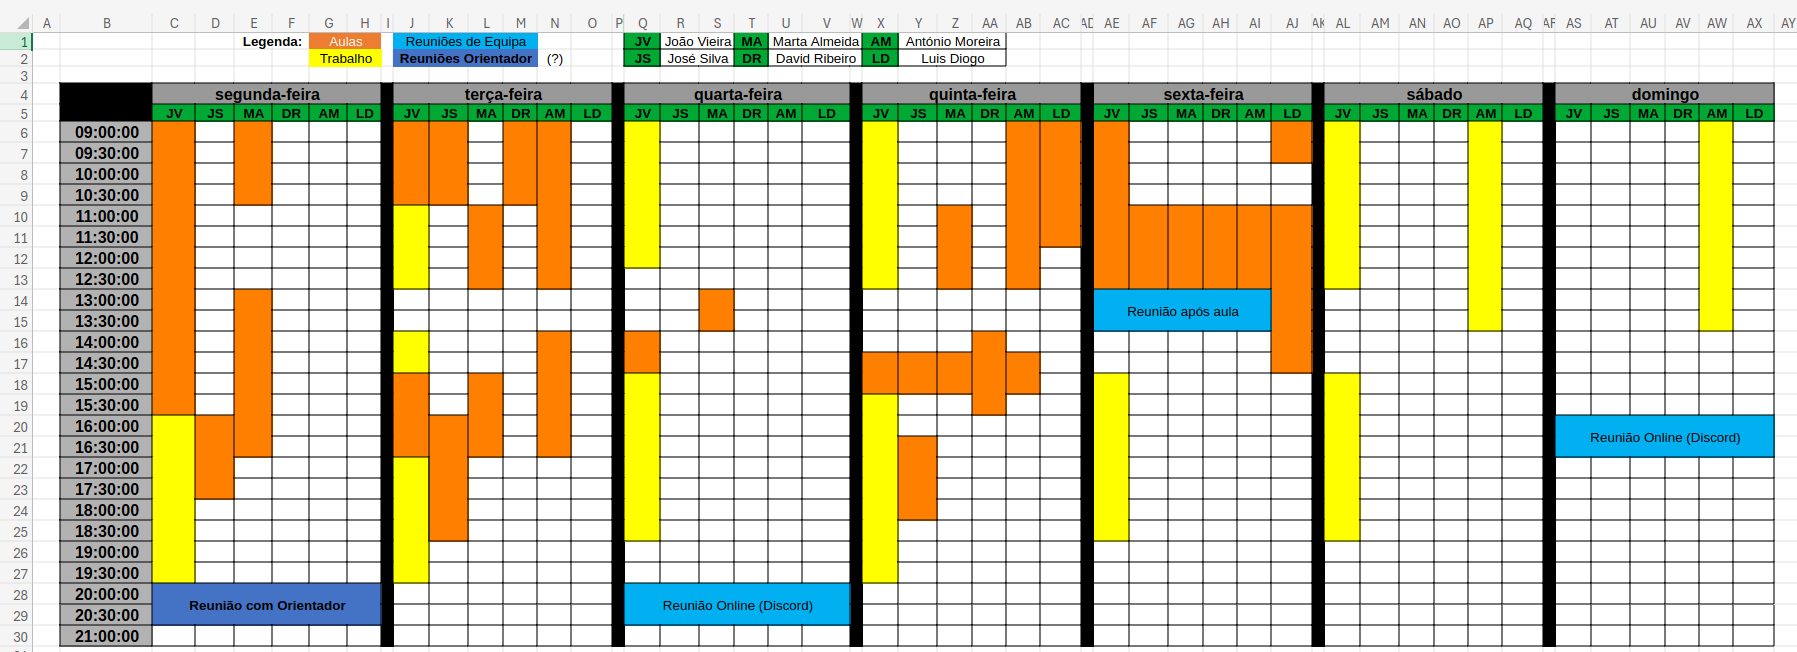
\includegraphics[width=16cm]{figs/team_schedule.png}
      \caption{Team schedule and meeting planner implemented in Excel, showing member availability, scheduled meetings, and project milestones}
      \label{fig:schedule}
\end{figure}

\section{Team Structure and Roles}
\label{section:team_structure} 

Effective project management and execution rely heavily on a well-defined team structure with clear roles and responsibilities. This section outlines the organizational framework adopted for this project, designed to optimize workflow, foster specialization, and ensure comprehensive coverage of all project aspects. 

\subsection{SCRUM Master}
\label{subsec:scrum_master} 
The team member, João Vieira, has been appointed as the \textit{SCRUM Master} for this project. In this pivotal role, he will: 

\begin{itemize}
    \item Facilitate the SCRUM process
    \item Ensure adherence to SCRUM principles and practices
    \item Remove obstacles impeding team progress
    \item Foster an environment of continuous improvement
\end{itemize} 

\subsection{Sub-teams}
\label{subsec:sub_teams} 

To enhance efficiency and leverage individual strengths, the project team has been divided into three specialized sub-teams:

\subsubsection{Team Nº1: Frontend Development Team}
\begin{itemize}
    \item \textbf{Team Leader:} José Silva 
    \item \textbf{Members:} José Silva \& Marta Almeida
    \item \textbf{Responsibilities:}
    \begin{itemize}
        \item Designing and implementing user interfaces.
        \item Creating responsive and interactive layouts.
        \item Developing and maintaining client-side applications.
        \item Ensuring cross-browser and cross-platform compatibility and optimal performance.
        \item Collaborating with backend team to integrate user-facing elements.
        \item Implementing user experience best practices.
        \item Optimizing applications speed and scalability.
    \end{itemize}
\end{itemize} 

\subsubsection{Team Nº2: Backend Development Team}
\begin{itemize}
    \item \textbf{Team Leader:} João Vieira 
    \item \textbf{Members:} João Vieira \& David Ribeiro
    \item \textbf{Responsibilities:}
    \begin{itemize}
        \item Developing and maintaining server-side logic.
        \item Designing and managing databases.
        \item Creating and optimizing database.
        \item Implementing security measures.
        \item Developing APIs for frontend and third-party integrations.
        \item Ensuring scalability and performance of server-side applications.
        \item Collaborating with frontend team to integrate server-side logic.
        \item Monitoring and optimizing system performance.
    \end{itemize}
\end{itemize}

\subsubsection{Team Nº3: Research and Development Team}
\begin{itemize}
    \item \textbf{Team Leader:} António Moreira 
    \item \textbf{Members:} António Moreira \& Luís Diogo
    \item \textbf{Responsibilities:}
    \begin{itemize}
        \item Conducting in-depth research on emerging technologies and industry trends.
        \item Developing innovative solutions to address complex project challenges.
        \item Prototyping and testing new features or functionalities.
        \item Providing technical support and expertise to other teams as needed.
        \item Collaborating with frontend and backend teams to integrate research findings.
        \item Evaluating and recommending new tools or methodologies to enhance project efficiency.
    \end{itemize}
\end{itemize}

This strategic division allows each sub-team to focus on specific project aspects while maintaining overall cohesion through regular communication and collaboration. The structure is designed to promote expertise development, streamline workflows, and ensure comprehensive coverage of all project requirements.


\section{Risk Analysis and Mitigation Strategies}
\label{section:risk_analisys_mitigation_strategies}

The implementation of all of SPLASH's technologies brings innately some risks.

System reliability is a crucial concern, such as hardware malfunctions, battery failures, or connectivity failures. To mitigate this, pre-deployment testing, hardware redundancy, such as having backup devices, and regular, scheduled maintenance should be a priority and focus of anyone actively using the SPLASH system.\\

Weather conditions and environmental events can impact the usage and effectiveness of multiple equipment. To address this, equipment with higher environmental durability should be selected. With high quality equipment and contingency protocols in place, all potential climate-related risks are minimized.\\

It is also worthy of mention that human error is a factor, and not all people adapt fast to new technologies. Having a user-friendly design minimizes the friction one may feel while getting used to the SPLASH system. Giving lifeguards the proper training required should also be a high priority matter.\\




%%
\begin{thebibliography}{9}

\bibitem{infopraia1} 
Info Praia.
\textit{Informação sobre as praias portuguesas.}
Disponível em: \url{https://infopraia.apambiente.pt/about/}, acedido em 12/11/2024.

\bibitem{infopraia2} 
Sistema Nacional de Informação de Recursos Hídricos.
\textit{Info Praia - Informações detalhadas sobre praias.}
Disponível em: \url{https://snirh.apambiente.pt/index.php?idMain=1&idItem=2.1}, acedido em 12/11/2024.

\bibitem{praia5g1} 
Costa da Caparica: Primeira Praia com Cobertura 5G.
\textit{SAPO Tek - Notícias sobre telecomunicações.}
Disponível em: \url{https://tek.sapo.pt/noticias/telecomunicacoes/artigos/costa-da-caparica-e-a-primeira-praia-portuguesa-com-cobertura-5g}, acedido em 14/11/2024.

\bibitem{praia5g2} 
NOS.
\textit{Primeira Praia 5G - Casos de inovação.}
Disponível em: \url{https://www.nos.pt/5g/5g-em-acao/casos-de-inovacao/primeira-praia-5g}, acedido em 14/11/2024.

\end{thebibliography}
\end{document}